\section{Mais quelle est donc cette matière ? (4 points)}

Nolan ne se rappelle plus quel plastique il doit acheter pour son imprimante 3D : de l'ABS ou du PLA ?

\begin{itemize}
	\item \textbf{L'ABS} est un plastique courant, on le retrouve dans les Lego par exemple. Son point fort vient de sa solidité, il commence à fondre à 180°C.
	
	\item Issu de matériaux recyclés, tels que l'amidon de maïs \textbf{le PLA} est une matière plus naturelle et biodégradable. Sa température de fusion est de 160°C.	
\end{itemize}

\begin{questions}
	\question[2] Quelle expérience Nolan peut-il réaliser pour identifier le plastique de son imprimante ?
	
	\question[2] Il trace l'évolution de la température pendant la fusion du plastique. Quel est le plastique de son imprimante ?
	
	\begin{center}
		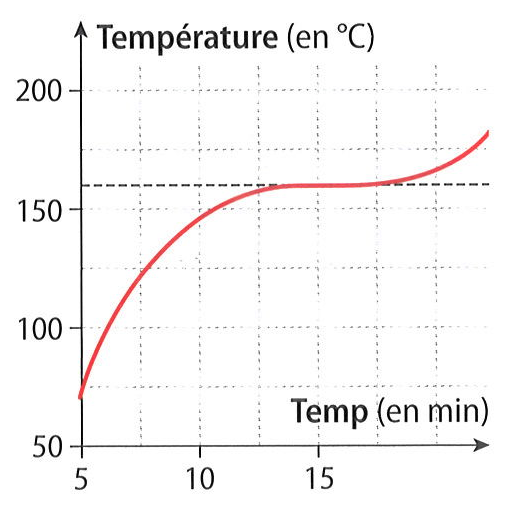
\includegraphics[scale=0.6]{img/courbe2}
	\end{center}
\end{questions}